% !TeX spellcheck = it_IT
\section{Mobile Network}

\subsection{Introduzione alle reti mobili}

\paragraph{Pre-Cellulare:} Prima degli anni '80 esistenza un servizio di telefonia mobile con trasmettitori e ricevitori ad elevata potenza, con 25 canali e 80km di raggio di copertura. Capacità insufficiente per fornire un servizio di telefonia (voce) comparabile con i servizi di telefonia fissi.\\

L'idea dietro la rete cellulare invece è usare \textbf{molteplici trasmettitori} con una potenza "bassa", minore di 100W. Meno potenza, meno raggio di copertura: l'area viene divisa in celle (da qui "cellulare"), ognuna con una propria antenna (o più).\\

Ogni cella è servita da una \textbf{Base Station (BS)}:
\begin{itemize}
	\item Trasmettitore
	\item Ricevitore
	\item Unità di controllo
\end{itemize}
Può operare in licensed/unlicensed spectrum.\\

La progressione è:
\begin{itemize}
	\item 1980 \textbf{1G Advanced Mobile Phone Service (AMPS)}: Voce analogica in mobilità
	\item 1990 \textbf{2G Global System for Mobile Communication (GSM)}: Voce digitale (compressa, \dots), prima rete globale
	\item 2000 \textbf{3G Universal Mobile Telecommunications System (UMTS)}: Introduce i servizi internet
	\item 2010 \textbf{4G Long Term Evolution (LTE)}: convergenza IP e aumento delle prestazioni
	\item 2020 \textbf{5G}: Networks softwarization \& virtualization, slicing \& bassa latenza
	\item 2030 \textbf{6G}: Network intelligence (AI all'interno della rete, ottimizzazione secondo AI)
\end{itemize}

Gli standard della rete cellulare si possono vedere su \href{https://www.3gpp.org/specifications-technologies/releases}{\texttt{Third Generation Partnership Project (3GPP)}}. Sono tutte le release su cui si basano i rilasci commerciali.\\

\paragraph{Base Station BS:} Un esempio di BS può essere
\begin{center}
	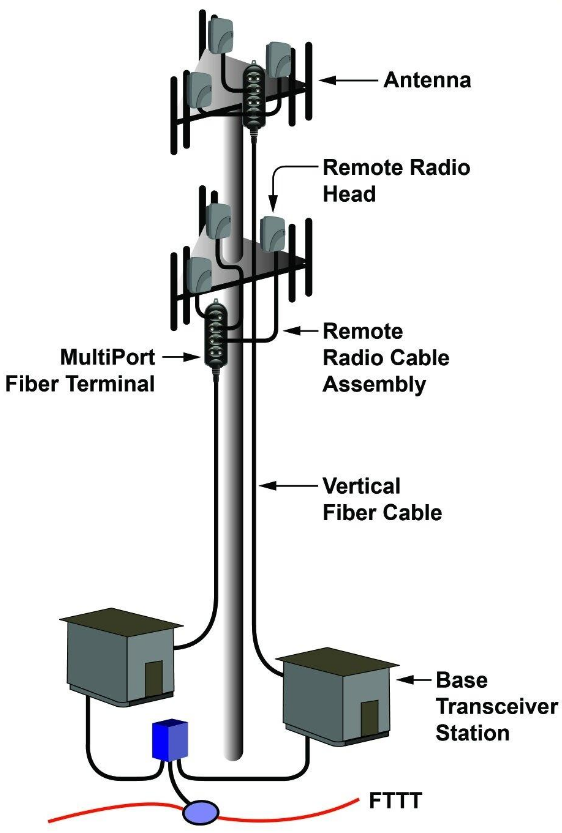
\includegraphics[width=0.4\linewidth]{img/mobile/1BS}
\end{center}

Le componenti sono:
\begin{itemize}
	\item \textbf{Antenna}: trasmette e riceve onde radio
	\item \textbf{Remote radio head}: riceve i segnali analogici e li converte in digitale e viceversa; vicino all'antenna per ridurre la perdita di segnale nei cavi
	\item \textbf{Remote radio cable assembly}: gruppo di cavi che fornisce alimentazione e/o collegamento dati tra la stazione base e i Remote Radio Heads
	\item \textbf{MultiPort Fiber Terminal}: punto di terminazione o distribuzione in cui la fibra ottica in entrata viene divisa o collegata a più uscite per servire le diverse RRH. In pratica, funge da "scatola di giunzione" per organizzare e connettere i vari cavi in fibra destinati ai moduli radio remoti
	\item \textbf{Base Transceiver Station (BTS)}:L'elemento principale dell'infrastruttura della rete mobile, gestisce il traffico dati e vocale, coordina i protocolli radio, si interfaccia con la rete di trasporto verso il core network dell'operatore e invia i segnali digitali agli RRH. Al suo interno si trova l'elettronica di baseband (elaborazione del segnale, modulazione/demodulazione, protocolli) e vari componenti di controllo
\end{itemize}

\subsection{Organizzazione Geometrica delle Celle}

Bisogna capire come disporre le celle. I requisiti sono:
\begin{itemize}
	\item coprire "bene" l'area
	\item avere una disposizione uniforme
\end{itemize}

Una buona disposizione usa celle esagonali per una copertura e disposizione uniforme. Ovviamente si tratta della disposizione ideale, nella realtà ci sono dei vincoli, di posizionamento e diffusione del segnale.\\

\paragraph{Riuso delle frequenze:} Si ha il problema di avere celle vicine con la stessa banda di frequenza: dispositivi sui bordi ricevono dati da entrambe le celle. \\

La prima soluzione è usare \textbf{frequenze diverse tra celle vicine}, ma servono più bande (licensed spectrum, costa e ne uso solo una parte per volta). 2G opera in questo modo.\\

Un'altra soluzione, per non "sprecare" banda, è usare la stessa frequenza e \textbf{tecniche di codifica} per evitare le interferenze tra celle vicine (\textbf{CDMA}).\\

L'ultima soluzione è:
\begin{itemize}
	\item al \textbf{centro} di ogni cella usare l'\textbf{intera ban}da disponibile (tranne un pezzo), per gli utenti interni
	\item al \textbf{bordo}, \textbf{celle vicine} hanno \textbf{frequenze diverse}
\end{itemize}

Questo permette bandwidth maggiore per utenti interni ma richiede un sofisticato controllo di potenza e coordinamento tra BS (4G e 5G). Bisogna posizionare all'interno della cella i dispositivi in maniera abbastanza precisa per stabilire che frequenze utilizzare. \\

%fino s16
%End L15

\newpage

\subsubsection{Aumento della capacità per migliorare la scalabilità}
 
Uno degli obiettivi fondamentali delle reti cellulari è servire sempre più utenti utilizzando lo spettro disponibile (costo elevato), evitando di utilizzare ed installare troppe BS. La rete cellulare è formata da celle, e una BS può contenere più celle.\\ 

Una gestione dinamica delle frequenze tra celle vicine permetterebbe il prestito di frequenze, con i relativi costi di sincronizzazione.\\

Si possono aumentare le celle, suddividendole e rendendole più dense in aree con più elevato traffico, ma più celle ci sono più è frequente il cambio di cella (handoff/handover), con il relativo traffico di controllo.\\

\paragraph{Cell sectoring:} Una BS può avere diverse antenne direzionali (al posto di una omnidirezionale) che permettono di creare diverse celle
\begin{center}
	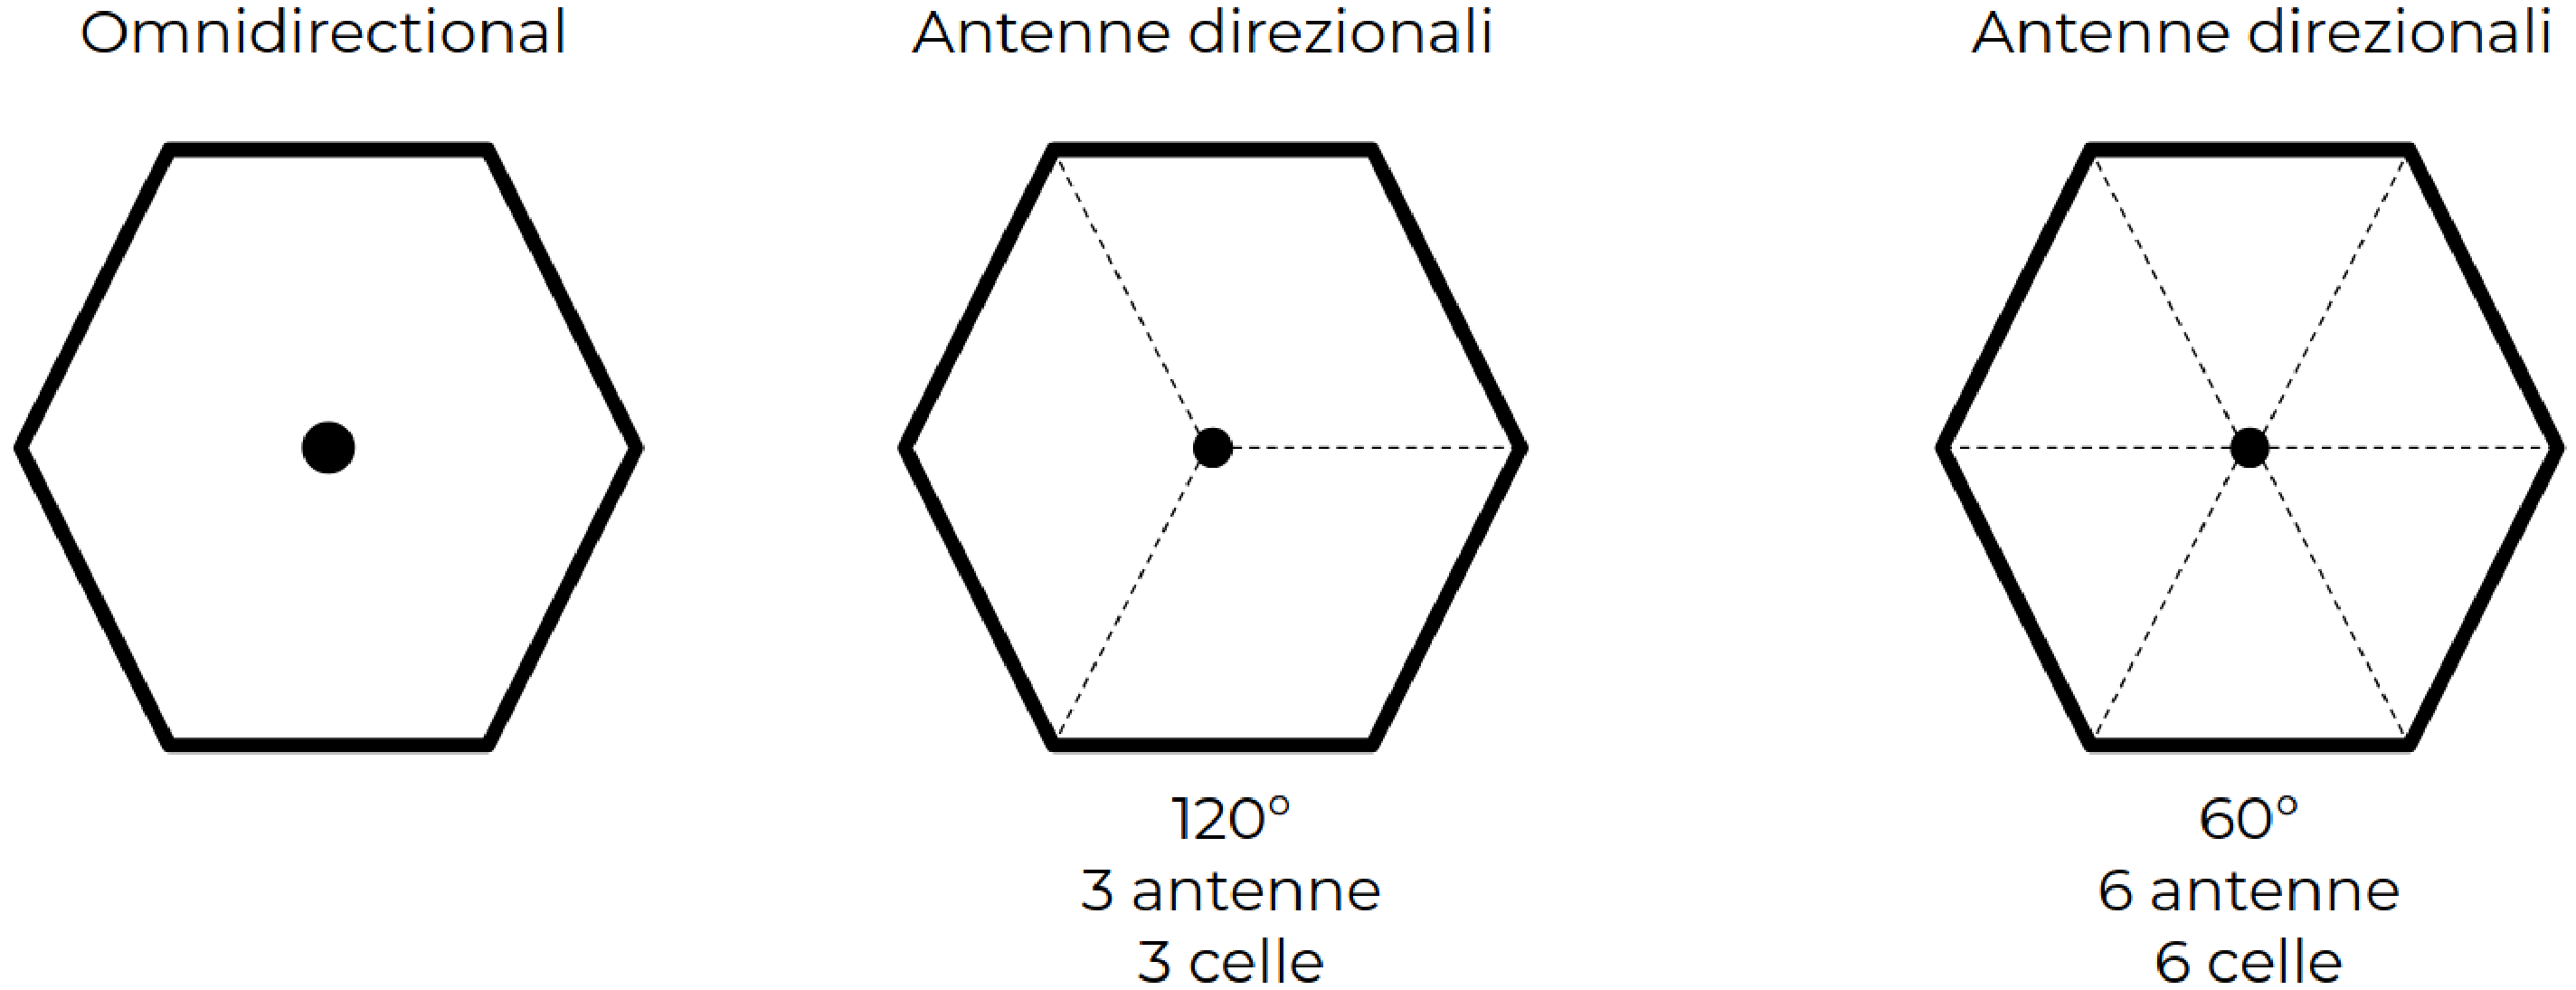
\includegraphics[width=0.8\linewidth]{img/mobile/sectoring}
\end{center}

Sono effettivamente celle diverse, con i relativi problemi di bordo e handover, ma restringere la cella permette di migliorare il data rate. Dare una direzionalità di gain molto alta permette di ridurre il path loss (\textbf{Beamforming}).\\

\newpage

\subsection{Architettura}

L'architettura di una rete cellulare si divide in grosse macro aree: 
\begin{itemize}
	\item \textbf{Radio Acces network RAN}: la parte di stazioni e collegamento radio che forniscono collegamento ai dispositivi mobili
	\item \textbf{Core Network}: la parte centrale responsabile della gestione e del controllo della comunicazione tra utenti e servizi esterni
\end{itemize}
\begin{center}
	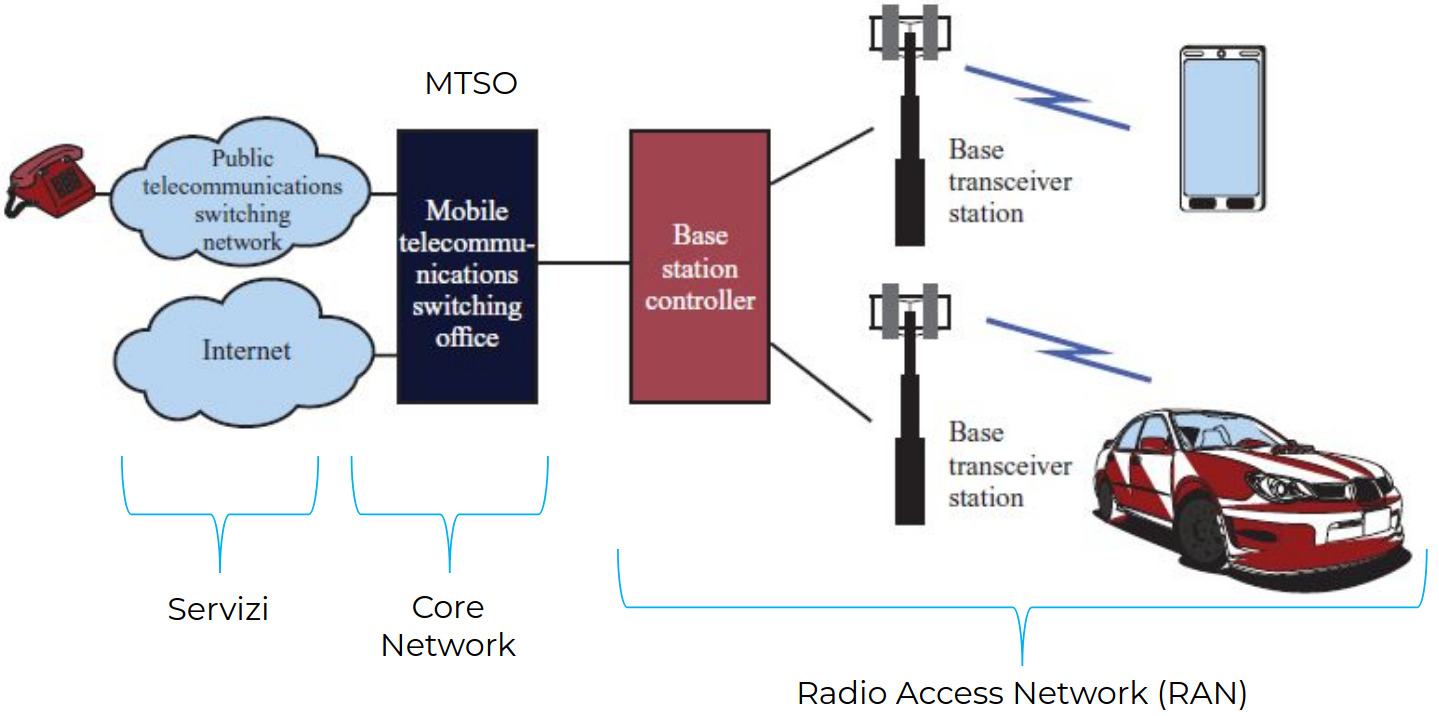
\includegraphics[width=0.8\linewidth]{img/mobile/archop}
\end{center}
Tutto il core network è rete fissa, fino alle antenne, per poi essere wireless. \\
%Boh, compl
Tutte le operazioni delle rete cellulare sono automatiche e non richiedono alcun intervento da parte dell'utente. Si ha una separazione netta tra quelli che sono i canali di controllo, fisici o virtuali. \\

Esistono \textbf{2 tipi di canali} che trasportano 2 tipologie di traffico:
\begin{itemize}
	\item \textbf{Canali di controllo}: trasportano tutte le informazioni per la gestione delle operazioni, \textbf{Control Plane} (es. handoff, autenticazione, \dots)
	\item \textbf{Canali di traffico}: trasportano voce e dati (traffico dei servizi offerti all'utente), \textbf{Data Plane}
\end{itemize}
Si ha una divisione Control/Data plane netta ed esplicita.\\

\newpage

\subsection{Operazioni}

\paragraph{Inizializzazione:} Ci sono diverse funzionalità. Si ha una fase di inizializzazione che serve a capire i segnali che vengono ricevuti, il dispositivo utente monitora i segnali delle celle per identificare quella migliore. Periodicamente ogni BS invia dei \textbf{pilot} che permettono al dispositivo di determinare la qualità del segnale di quella cella.\\

Quando un dispositivo vuole iniziare una comunicazione con la rete cellulare:
\begin{enumerate}
	\item \textbf{Disponibilità di canali radio con BS}: ascolta le trasmissioni broadcast delle BS per individuare quale cella ha segnale sufficiente, quali canali radio sono liberi e quali parametri di accesso usare
	\item \textbf{Traffico di controllo per iniziare la comunicazione con MTSO}: viene inoltrata la richiesta di comunicazione, fino al MTSO, che si occupa di autenticare l'utente, verificare permessi e risorse, decidere se e come procedere (Core network)
	\item \textbf{Creazione dei "collegamenti" su data plane}: se la fase di controllo va a buon fine, vengono allocati i canali fisici e logici necessari per il traffico dati, il dispositivo potrà cominciare a scambiare dati liberamente
\end{enumerate}

\paragraph{Paging:} L'operazione di pagine è il "cercare" il dispositivo, perché c'è \textit{qualcosa} che deve raggiungerlo. I device non sono sempre attivi nella rete cellulare, quindi potrebbe essere necessario cercarli. Il dispositivo si può muovere in completa libertà, è \textbf{compito della rete} "ritrovare" la posizione quando necessario.\\

MTSO non è sempre a conoscenza della posizione del dispositivo (ovvero la cella a cui è associato), il dispositivo può essere in idle mode (senza una connessione attiva). MTSO quindi contatta le BS delle celle per "trovare" il dispositivo.\\

\newpage

\paragraph{Chiamata accettata:} La chiamata (in realtà i dati, si parla in generale) passa \textbf{sempre} attraverso il core network:
\begin{itemize}
	\item Il dispositivo destinatario accetta la chiamata
	\item MTSO crea un circuito (fino a 3G, da 4G VoIP)
	\item le BS impostano i canali radio data plane
\end{itemize}

Durante una chiamata I due dispositivi si scambiano informazioni attraverso le BS a cui sono collegate e MTSO. In realtà, oltre a up e down link, può esistere il side link: un meccanismo che permette di bypassare BS e (in parte) core network per la comunicazione; nasce per scenari Device-to-Device D2D e Vehicle-to-Everything V2X.\\

\paragraph{Handoff:} I dispositivi possono muoversi al di fuori del raggio della cella nella quale hanno iniziato la comunicazione. Serve collegarsi ad un'altra cella; le fasi sono:
\begin{enumerate}
	\item Decisione di nuova associazione
	\item Gestione nuova associazione
	\item Riconfigurazione percorsi di comunicazione
\end{enumerate}

Il tutto deve avvenire in maniera \textbf{automatica} e \textbf{senza interruzione della comunicazione} (entro certi limiti della tecnologia, ad esempio meno di 200km/h).\\

\newpage

\subsection{Ambiente}

Il contesto nel quale la rete cellulare opera è molto più dinamico e imprevedibile degli altri scenari wireless. Contesti \textbf{molto eterogenei} e molto complessi. \\

La \textbf{potenza del segnale} deve essere: 
\begin{itemize}
	\item sufficiente per offrire un servizio di buona qualità
	\item non troppo per non creare interferenza
	\item molto variabile per via degli ostacoli
\end{itemize}

Il \textbf{fading} (attenuazione del segnale) dipende anche da frequenza e tipo di ambiente.\\

\subsubsection{Deployment}

Gli operatori di rete mobile pianificano con molta attenzione l'installazione delle BS al fine di ottimizzare la rete. Operazione chiamata Network Planning. Questo include:
\begin{itemize}
	\item Posizionamento delle BS
	\item Dimensionamento delle BS
	\item Rete di trasporto verso MTSO
	\item Bande da utilizzare (frequenze più basse maggiore copertura, bandwidth limitata, frequenze più alte maggiore bandwidth, minore penetrazione ostacoli)
\end{itemize}

\newpage

\subsection{Handoff/Handover}

Uno degli aspetti più rilevanti è la \textbf{gestione dell'handover}, ovvero il cambio da una cella all'altra. La procedura può essere decisa in due modi:
\begin{itemize}
	\item \textbf{solo dalla rete}: basata sulla misurazione del segnale ricevuto dal dispositivo (uplink)
	\item \textbf{dispositivo coinvolto nella decisione}: fornisce un feedback sul segnale percepito (downlink)
\end{itemize}
Diverse metriche vengono monitorate dalle BS per prendere una decisione, ma il parametro principale per la decisione è la potenza del segnale ricevuta a livello di BS (e dal dispositivo coinvolto).\\

Il metodo più semplice è guardare \textbf{solo la potenza relativa}: l'associazione viene fatta alla BS che ha il migliore segnale. Ma l'handover è una procedura costosa e il segnale potrebbe fluttuare (ad esempio sui bordi della cella), portando all'effetto ping pong, ovvero un cambio continuo tra le BS. Questo può essere parzialmente risolto tenendo sul device uno storico delle BS a cui si è collegato, evitando di ri-collegarsi a BS da cui è stato fatto handover di recente.\\

Il primo miglioramento può essere \textbf{introdurre una soglia}: se il segnale è abbastanza buono (oltre una soglia), perché cambiare? L'handover ora viene effettuato solo nel caso il segnale sia peggiore di un'altra BS ma deve anche essere sotto una certa soglia. Si ha il problema di definire queste soglie, in quanto dipendono da diverse condizioni di contesto.\\

\newpage

Un altro miglioramento è aggiungere \textbf{isteresi}: si tiene un margine, per far partire l'handover deve esserci una differenza significativa di potenza. 
\begin{center}
	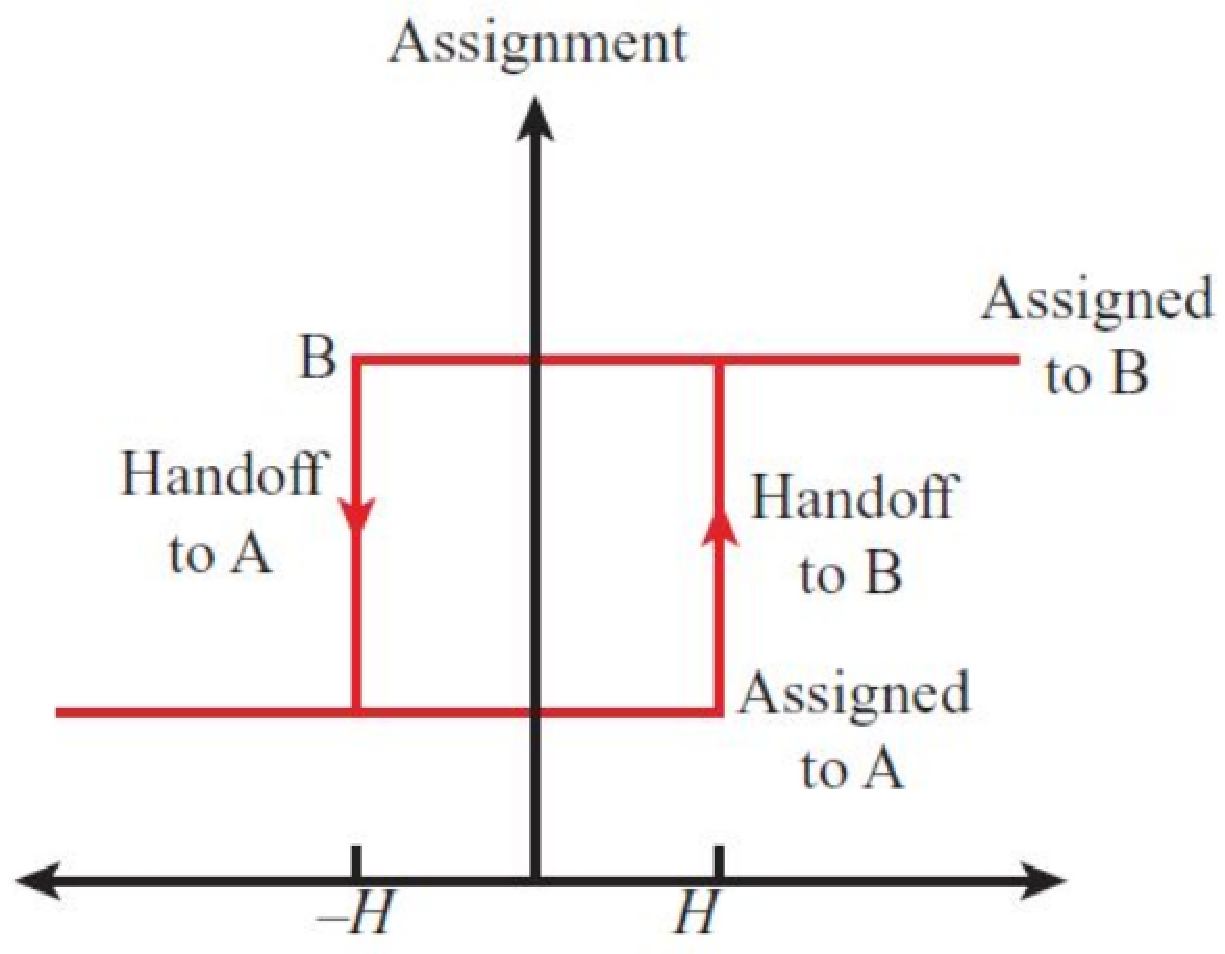
\includegraphics[width=0.55\linewidth]{img/mobile/isteresi}
\end{center}

Risolve il Ping-Pong ma rimane il problema che il segnale della prima BS può essere ancora "abbastanza buono". Si possono \textbf{combinare le idee}, per determinare l'handover si usano 
\begin{itemize}
	\item \textbf{potenza relativa}: deve essere abbastanza grande
	\item \textbf{soglia}: il segnale deve essere abbastanza "brutto"
	\item \textbf{isteresi}: la differenza deve essere significativa
\end{itemize}

\paragraph{Hard vs Soft Handoff:}
\begin{itemize}
	\item \textbf{Hard handoff}:
	\begin{itemize}
		\item il dispositivo è associato ad una sola BS alla volta
		\item cambio immediato di frequenza per agganciarsi alla BS vicina
		\item protocolli di handoff vicini
	\end{itemize}
	
	\item \textbf{Soft handoff}
	\begin{itemize}
		\item il dispositivo mantiene la connettività con entrambe le BS
		\item il rilascio di una BS quando il segnale è chiaramente dominante
		\item richiede più risorse in quanto il dispositivo è allocato più volte
	\end{itemize}
\end{itemize}

\newpage

\subsection{Duplex}
Per la gestione del duplex ci sono 2 modalità:
\begin{itemize}
	\item \textbf{Frequency Division Duplex FDD}: utilizzo di frequenze diverse per uplink e downlink; minore delay, maggiori risorse richieste
	\item \textbf{Time Division Duplex TDD}: una sola frequenza sia per uplink che downlink, maggiore ritardo perché bisogna aspettare
\end{itemize}

\subsection{GSM Mobile Station (MS)}

Si intende un dispositivo, cambia un po' nome attraverso alle generazioni ma sempre terminale finale si intende. In generale la struttura è
\begin{center}
	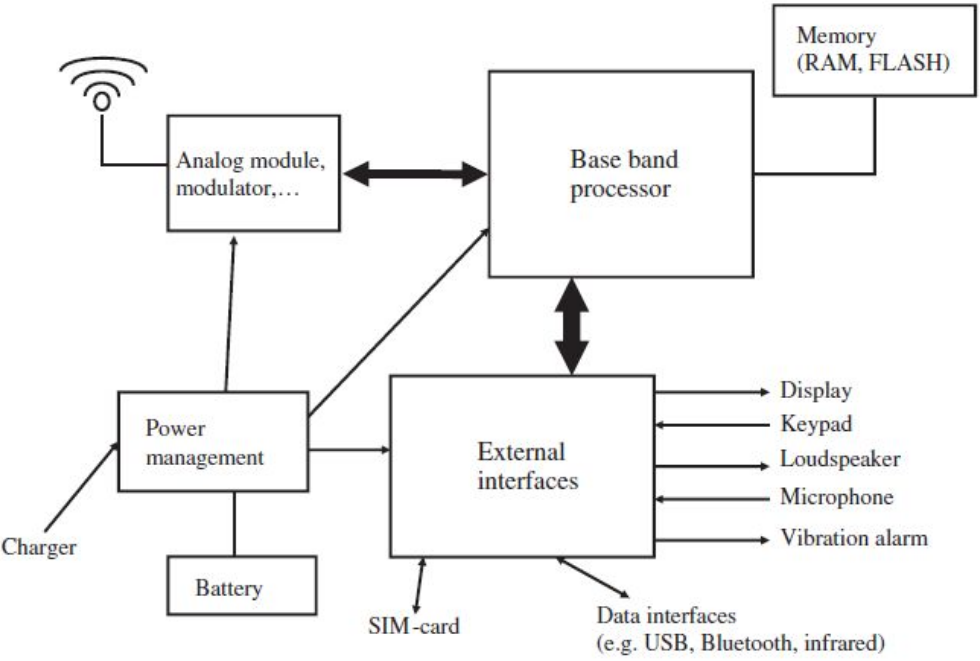
\includegraphics[width=0.65\linewidth]{img/mobile/ms1}
\end{center}

Ogni dispositivo (solo terminale mobile) possiede un identificativo unico detto \textbf{Internetional Mobile Equipment Identiity IMEI} (15 cifre). Hanno struttura
\begin{center}
	%\renewcommand{\arraystretch}{1.4}
	\begin{tabular}{| >{\centering\arraybackslash}m{3cm} | >{\centering\arraybackslash}m{2cm} | >{\centering\arraybackslash}m{3cm} | >{\centering\arraybackslash}m{2cm} |}
		\hline
		\textbf{TAC (6)} & \textbf{FAC (2)} & \textbf{SN (6)} & \textbf{Check digit (1)} \\
		\hline
		Type Approval Code, Codice del costruttore & 
		Final Assembly Code, Luogo costruzione & 
		Numero seriale & 
		Numero di controllo di validità del codice \\
		\hline
	\end{tabular}
\end{center}

Identificano a livello mondiale ogni dispositivo mobile.\\

\newpage

\subsubsection{SIM Card}

La SIM contiene informazioni per \textbf{identificare l'utente} (abbonato) e la chiave segreta per autenticazione e generazione chiavi di cifratura, reti preferite e proibite, PIN, PUK, ultime location, ecc.\\

Si hanno diversi formati, di diverse dimensioni, fino a Embedded SIM (eSIM), un chip programmabile all'interno del dispositivo.\\

Ha un \textbf{International Mobile Subscriber Identity IMSI} (diverso dal numero di telefono), il quale identifica una specifica SIM card (max 15 cifre).\\

Il numero di telefono viene chiamato \textbf{Mobile Subscriber Integrated Service Digital Number MSISDN}. Struttura:
\begin{center}
	\begin{tabular}{| >{\centering\arraybackslash}m{2cm} | >{\centering\arraybackslash}m{2cm} | >{\centering\arraybackslash}m{4cm} | }
		\hline
		\textbf{CC} & \textbf{NDC} & \textbf{Numero} \\
		\hline
		Country CODE & Network Destination Code & Numero utente \\
		\hline
		+39 & 123  & 1234567 \\
		\hline
	\end{tabular}
\end{center}

Si può avere l'associazione 1:1 tra SIM e numero di telefono, oppure un'associazione 1:N. Funzionalità per la portabilità del numero telefonico. \\

Il campo NDC, dopo l'introduzione della portabilità del numero, non ha più senso, non rappresenta più l'operatore.\\

%%%%%%%%%%%%%%%%%%%%%%%%%%%%%%%%%%%%%%%%%%%%%
% STORY TIME %
%%%%%%%%%%%%%%%%%%%%%%%%%%%%%%%%%%%%%%%%%%%%%

\newpage

\subsection{Story Time: Prima del 4G}

\subsubsection{Global System for Mobile Communications GSM}

Standard sviluppato all'inizio degli anni '90. Inizialmente la trasmissione dati era di tipo Circuit Switched (principalmente voce, ogni chiamata aveva una linea dedicata).  Riutilizzava tecnologie preesistenti, principalmente per la telefonia fissa, adattate pe rla rete mobile. All'inizio la trasmissione era analogica, dalla seconda metà degli anni '80 la voce comincia ad essere digitalizzata.\\

Dalle prime versioni di GSM circuit-switched si è progressivamente passati a soluzioni basate su Virtual Circuit Switching over IP (da commutazione di circuito a soluzioni IP-based). Si crea un "circuito virtuale" con una connessione logica temporanea su una rate IP. Risorse allocate in modo bidirezionale per tutta la durata del servizio.\\


Viene standardizzato dall'ETSI (European Telecommunication Standard Institute), prima a livello europeo, poi mondiale. Si tratta della prima volta in cui sono presenti standard comuni. Da UMTS in poi la standardizzazione è affidata a 3GPP.\\

Come si trasmette? Interfaccia radio tra device e base station è denominata Um ("U mobile", da ISDN). Usa Frequency Division Duplex (FDD), 2 bande attorno ai $900MHz$, $25MHz$ ognuna. Ogni banda è divisa in 125 canali da $200kHz$. \\

Una singola cella può avere estensione fino 35km (teoricamente, molto meno nella pratica). Suddivisione in celle e settori più piccoli permette di aumentare la capacità. Si ha una pianificazione del riuso delle frequenze in base alla posizione delle celle.\\

GSM implementa il multiple access usando due tecniche: 
\begin{enumerate}
	\item FDMA (divisione in frequenza): Divide lo spettro disponibile in canali da $200 kHz$, con 125 canali per direzione (Uplink e Downlink, $25MHz$ ciascuno). Tuttavia, non tutti i canali possono essere usati in ogni cella per evitare interferenze tra celle vicine
	\item TDMA (divisione temporale): ogni canale in frequenza può essere diviso in 8 slot temporali, permettendo l'accesso a 8 dispositivi tramite turni di trasmissione
\end{enumerate}

La trasmissione duplex non è possibile, i dispositivi devono alternare la trasmissione e la ricezione, richiede tempo. \\

\subsubsection{General Packet Radio Service GPRS \& Enhanced Datarates for GSM Evolution EDGE}

La rete GSM è perfetta per trasportare traffico voce: 
\begin{itemize}
	\item bit rate costante
	\item risorse pre-allocate e riservate (Time slot TDM diverso per ogni utente)
	\item delay costante (time slot TDM)
	\item No overhead di informazioni per segnalazione
	\item Tariffazione a durata (pago minuti/scatti)
\end{itemize}
ma anche per trasportare SMS:
\begin{itemize}
	\item Servizio delay-tolerant su canale di segnalazione
	\item Contenuto testuale semplice
	\item Tariffazione per SMS
\end{itemize}

Ma la rete GSM è idonea per offrire un servizio dati internet? 
\begin{itemize}
	\item Il traffico dati Internet ha un data rate variabile e l'interazione è intermittente e a burst
	\item Circuit-switched non è ottimale:
	\begin{enumerate}
		\item Le risorse pre-allocate sono inutilizzate per molto tempo
		\item Allocazione fissa non compatibile con traffico dati Internet
		\item Le risorse non utilizzate sono sprecate e non utilizzabili da altri utenti
	\end{enumerate}
	\item La tariffazione a durata non ha molto senso con dati Internet
\end{itemize}

GPRS è una rete a pacchetto (packet switched) realizzata come overlay (RAN) e aggiunta (Core) della rete GSM. Cerca di mantenere fissa la parte di RAN e Core per adattarla all'uso di internet. Permette: 
\begin{itemize}
	\item Data rate per utente di $20kbps$ ($270kbps$ EDGE)
	\item Tariffazione a volume di traffico
	\item Rilascio degli slot in idle (per natura burst del traffico)
	\item "Ridotto" tempo di connessione ad internet (da 20s GSM a 5s GPRS)
	\item La connessione (logica) non viene rilasciata, vengono rilasciati solo i time-slot radio; libera le risorse radio, mantiene l'IP associato
	\item La connessione (logica) è indipendente dalla connessione fisica, la mobilità o la perdita di copertura non interrompe la connessione
\end{itemize}

\subsubsection{GPRS Tunneling Protocol GTP}

Il GTP risolve il problema della mobilità per IP: dove invio i pacchetti se il dispositivo continua a muoversi? Non è possibile aggiornare le tabelle di routing ad ogni cambio della rete.\\
La connessione logica tra MS e GGSN è identificata da una sessione del protocollo Packet Data Protocol (PDP). MS è libero di muoversi all'interno della rete e possiede un proprio IP unico all'interno della rete (DHCP/NAT) e mantenuto per tutta la durata della sessione.\\

La soluzione è creare tunnel virtuali tra nodi della rete mobile, incapsulare il pacchetto, fornire un Tunnel End Point ID TEID, GTP realizza tunneling sopra al livello di trasporto. \\

\subsubsection{Universal Mobile Telecommunication System UMTS}

La velocità della rete fissa è aumentata, quindi in mobilità si vuole offrire accesso a Broadband Internet, oltre che gestione senza interruzione tra celle UMTS e GSM/GPRS, retro-compatibilità.\\

Viene cambiata la rete di accesso (UTRAN, UMTS Terrestrial Radio Access Network):
\begin{itemize}
	\item nuovo modello di architettura della BS
	\item nuovo concetto di canale radio (Radio Access Bearer RAB)
	\item Utilizzo di Code Division Multiple Access (CDMA)
	\item Maggiore banda per canale (da $200kHz$ a $5MHz$)
\end{itemize}

Vengono separate nettamente le funzionalità di segnalazione tra rete core e RAN:
\begin{itemize}
	\item Access Stratum (AS): Responsabile della gestione dei canali radio e della comunicazione tra il terminale e la rete.
	\item Non-Access Stratum (NAS): Gestisce le funzioni di mobilità, autenticazione e gestione della sessione tra l'utente e la rete core
\end{itemize}

Inoltre UMTS mantiene la compatibilità con le reti GSM e GPRS esistenti, per non richiedere cambiamenti radicali dell'infrastruttura.\\

\paragraph{CDMA:} Riuso totale delle frequenze, ogni cella usa le stesse frequenze, i codici ortogonali permettono di "eliminare" interferenza. Rispetto a GSM/GPRS, CDMA offre una trasmissione più fluida con latenze ridotte. CDMA è particolarmente resistente alle interferenze multipath. Grazie all'assegnazione di codici unici a ciascun utente, CDMA offre maggiore privacy. Inoltre, si tratta di un sistema altamente scalabile.\\

Il numero di chip è variabile in funzione della quantità di traffico che deve essere trasmessa e quanti utenti sono connessi.\\

Nel sistema GSM/GPRS, i canali erano definiti in base alla loro funzione e la loro posizione nello scheduling era predefinita e statica. Ogni canale aveva un compito specifico e non poteva essere adattato.  In UMTS, invece, i canali radio sono dinamici e vengono definiti attraverso una serie di parametri che ne determinano le caratteristiche. \\

Viene introdotta la nozione di Radio Access Bearer (RAB), cioè un canale radio che viene configurato in base a parametri specifici, tra cui:
\begin{itemize}
	\item Classe del servizio: Voce, streaming, interattivo, background
	\item Velocità massima: Indica la massima capacità di trasmissione del canale
	\item Velocità garantita: La velocità minima che il sistema assicura per la trasmissione dei dati
	\item Ritardo: Il tempo di latenza nella trasmissione dei dati.
	\item Probabilità di errore: Indica la qualità del canale in termini di errore nella trasmissione.
\end{itemize}

In UMTS ogni canale logico (dati/controllo) ha requisiti diversi, che vengono comunicati al sistema al momento della richiesta di connessione. \\

\subsubsection{HSDPA/HSUPA}

HSDPA è un'evoluzione della rete UMTS che migliora significativamente le velocità di download, ottimizzando l’uso delle risorse radio. Le tecnologie chiave dietro HSDPA sono:
\begin{itemize}
	\item Modulazione avanzata: Utilizza principalmente 16-QAM e 64-QAM
	\item MIMO (Multiple Input Multiple Output): sfrutta più antenne per migliorare la velocità e la stabilità della connessione
	\item Dual Carrier: Permette l'uso simultaneo di due portanti per raddoppiare la larghezza di banda disponibile.
\end{itemize}

Le diverse categorie di HS-DSCH (parametro) determinano il numero massimo di HS-PDSCH (High Speed Physical Downlink Shared Channel) utilizzabili simultaneamente e la velocità di trasmissione raggiungibile.\\

HSUPA è complementare a HSDPA (High-Speed Downlink Packet Access) e migliora la velocità in upload. Insieme, queste tecnologie formano HSPA (High-Speed Packet Access).\\

%End L16

\newpage